%!TEX TS-program = XeLaTeX
\documentclass[table,xetex,12pt,aspectratio=169]{beamer}
\usetheme{monokai}

\usepackage[english]{babel}
\usepackage{fontspec}
\setmainfont[Mapping=tex-text]{Source Serif Pro}
\setsansfont[Mapping=tex-text]{Source Sans Pro}
\setmonofont[Mapping=]{Source Code Pro}

\usepackage{minted}
\usemintedstyle{monokai}

\usepackage{tabularx}
\usepackage{tikz}
\usetikzlibrary{shapes.arrows}

\title{Introduction to x86-64 (dis)assembly}
\subtitle{aka. AMD64/x64}
\author{Toby Fleming}
\date{September 2016}

\AtBeginSection[]{\begin{frame}\vfill\centering\begin{beamercolorbox}[sep=8pt,center,shadow=false,rounded=false]{title}
\usebeamerfont{title}\insertsectionhead\par%
\end{beamercolorbox}\vfill\end{frame}}

\newcolumntype{Y}{>{\raggedleft\arraybackslash}X}
\newcolumntype{C}{>{\centering\arraybackslash}X}

\newcommand{\inputmintedtitle}[3][]{\inputminted[#1]{#2}{#3}{#3}}

\begin{document}

\maketitle

\begin{frame}{Note}
Talk only applies to executables that target SystemV AMD64 ABI. This means:
\vfill
\begin{itemize}
\item Unix (AIX, Solaris), Linux, FreeBSD/macOS
\item \textbf{not} Windows! (different ABI)
\item OS running on 64-bit, x86-compatible processors\\(most modern Intel/AMD processors)
\item ARM 64-bit (AArch64) ABI is also different!\\(e.g. Raspberry Pi, iOS)
\end{itemize}
\vfill
Also very much for beginners.
\end{frame}

\section{Registers}

\begin{frame}{Intel 8086}{16-bit, 1978}
\begin{tabularx}{\textwidth}{X<{\onslide<2->}|cc<{\onslide}}
 registers & Hi & Lo \\
\hline
AX (primary accumulator) & AH & AL \\
BX (base) & BH & BL \\
CX (counter) & CH & CL \\
DX (other functions, cba with backcronyms) & DH & DL \\
\hline
Index registers & 16-bit & only \\
\hline
SI (Source Index) & - & - \\
DI (Destination Index) & - & - \\
BP (Base Pointer) & - & - \\
SP (Stack Pointer) & - & - \\
\end{tabularx}
\vfill
\onslide<3->{And some more, not so important for now}
\end{frame}

\begin{frame}{Intel 80386}{32-bit, 1986}
\begin{tabularx}{\textwidth}{XXX}
32-bit & 16-bit & 8-bit \\
\hline
EAX & AX & AL \\
EBX & BX & BL \\
ECX & CX & CL \\
EDX & DX & DL \\
\hline
ESI & SI & - \\
EDI & DI & - \\
EBP & BP & - \\
ESP & SP & - \\
\end{tabularx}
\end{frame}

\begin{frame}{AMD Athlon 64}{64-bit, 2003}
\begin{tabularx}{\textwidth}{XXXXl}
64-bit & 32-bit & 16-bit & 8-bit & aka. \\
\hline
RAX & EAX & AX & AL & R0 \\
RBX & EBX & BX & BL & R1 \\
RCX & ECX & CX & CL &R2 \\
RDX & EDX & DX & DL &R3 \\
\hline
RSI & ESI & SI & SIL & R4 \\
RDI & EDI & DI & DIL & R5 \\
RSP & EBP & BP & BPL & R6 \\
RBP & ESP & SP & SPL & R7 \\
\hline
(\textbf{R}egister) & (\textbf{E}xtended) & & (\textbf{L}ow byte) & \\
\end{tabularx}
\end{frame}

\begin{frame}{AMD Athlon 64}{64-bit, 2003}
New general purpose registers R8--15!
\vfill
\begin{tabularx}{\textwidth}{XXXX}
64-bit & 32-bit & 16-bit & 8-bit \\
\hline
R8 & R8D & R8W & R8B \\
\multicolumn{4}{l}{\ldots} \\
R15 & R15D & R15W & R15B \\
\hline
(quadword) & (doubleword)* & (word) & (byte) \\
\end{tabularx}
\vfill
* Warning: aka. long word. This can be used in 32-bit asm instruction names (e.g. \texttt{movl}), and is why the new 8-bit registers don't use the \textbf{L} postfix.
\vfill\pause
\alert{Pop quiz: what's half a byte?}
\end{frame}

\begin{frame}{Register overlap}
\begin{tabularx}{\textwidth}{|XXXXXY|XY|XY|XY|}
63 & & & & & 32 & 31 & 16 & 15 & 8 & 7 & 0 \\
\multicolumn{12}{|c|}{\cellcolor{mediumgrey}RAX} \\
\multicolumn{6}{|c|}{} & \multicolumn{6}{c|}{\cellcolor{mediumgrey}EAX} \\
\multicolumn{6}{|c|}{} & \multicolumn{2}{c|}{} & \multicolumn{4}{c|}{\cellcolor{mediumgrey}AX} \\
\multicolumn{6}{|c|}{} & \multicolumn{2}{c|}{} & \multicolumn{2}{c|}{} & \multicolumn{2}{c|}{\cellcolor{mediumgrey}AL} \\
63 & & & & & 32 & 31 & 16 & 15 & 8 & 7 & 0 \\
\multicolumn{12}{|c|}{\cellcolor{mediumgrey}R8} \\
\multicolumn{6}{|c|}{} & \multicolumn{6}{c|}{\cellcolor{mediumgrey}R8D} \\
\multicolumn{6}{|c|}{} & \multicolumn{2}{c|}{} & \multicolumn{4}{c|}{\cellcolor{mediumgrey}R8W} \\
\multicolumn{6}{|c|}{} & \multicolumn{2}{c|}{} & \multicolumn{2}{c|}{} & \multicolumn{2}{c|}{\cellcolor{mediumgrey}R8B} \\
63 & & & & & 32 & 31 & 16 & 15 & 8 & 7 & 0 \\
\end{tabularx}
\end{frame}

\section{Calling conventions}

\begin{frame}{Calling conventions}
\begin{itemize}
\item Part of the ABI (Application Binary Interface, c.f. API)
\item Don't bother with x86 32-bit calling conventions: too many, inconsistent, old
\item ABI on most servers/desktops/laptops: SystemV AMD64
\item ...except Windows, ARM, very old 32-bit kit
\end{itemize}
\end{frame}

\begin{frame}{System V AMD64 ABI calling convention}
\begin{itemize}
\item First six integer args: RDI, RSI, RDX, RCX, R8, R9
\item Any more? Use stack
\item Floating point has other registers
\item Caller owns RBX, RBP, R12-R15
\item Called function must restore these if overwritten (use stack)
\item Return value in RAX (and RDX)
\end{itemize}
\vfill
Tedious, see handout!
\end{frame}

\section{Stack}

\begin{frame}{What's the call stack?}
\begin{columns}
\begin{column}{0.7\textwidth}
\alert{Warning, simplification!}
\begin{itemize}
\item last in, first out queue (push/pop)
\item way to ``allocate memory"
\item stack is limited in size and protected
\item use stack for local vars/short lived
\item use heap for large vars/long lived
\item stack grows downwards
\item heap grows upwards
\item ignore heap, managed by runtime (\texttt{malloc})
\end{itemize}
\end{column}
\begin{column}{0.3\textwidth}\pause
\begin{tikzpicture}[node distance=2cm,every node/.style={text=offwhite},arrow/.style={node distance=5cm,draw=offwhite,fill=orange,inner sep=10pt,shape=single arrow}]
\node (stack) [arrow,shape border rotate=270] {stack};
\node (heap) [below of=stack,arrow,shape border rotate=90] {heap};
\node [right of=stack] {e.g. 16 GiB};
\node [right of=heap] {0 GiB};
\end{tikzpicture}
\end{column}
\end{columns}
\end{frame}

\begin{frame}{What's the call stack?}
\begin{columns}
\begin{column}{0.5\textwidth}
\alert{Warning, simplification!}
\begin{itemize}
\item stack remembers program flow
\item each function has a stack frame
\item stack overflow = bad
\item can overwrite return address
\item boom, changed program execution
\end{itemize}
\end{column}
\begin{column}{0.5\textwidth}\pause
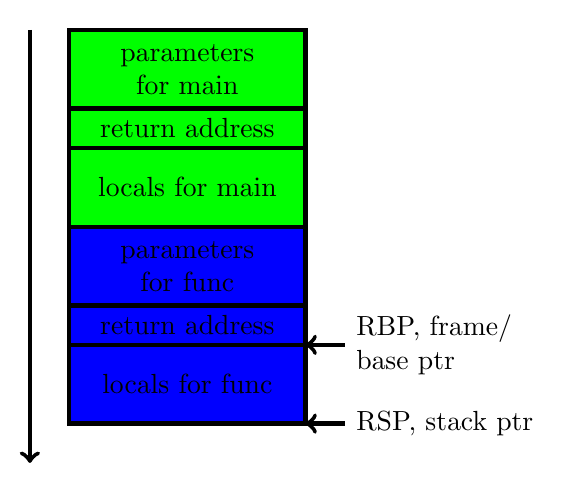
\begin{tikzpicture}[ultra thick]
\draw [fill=green] (0,0) rectangle (3,-1) node [midway,align=center] {parameters\\for main};
\draw [fill=green] (0,-1) rectangle (3,-1.5) node [midway] {return address};
\draw [fill=green] (0,-1.5) rectangle (3,-2.5) node [midway] {locals for main};
\draw [fill=blue] (0,-2.5) rectangle (3,-3.5) node [midway,align=center] {parameters\\for func};
\draw [fill=blue] (0,-3.5) rectangle (3,-4) node [midway] {return address};
\draw [<-] (3,-4) -- (3.5,-4) node [right,align=left] {RBP, frame/\\base ptr};
\draw [fill=blue] (0,-4) rectangle (3,-5) node [midway] {locals for func};
\draw [<-] (3,-5) -- (3.5,-5) node [right] {RSP, stack ptr};
\draw [->] (-0.5,0) -- (-0.5,-5.5);
\end{tikzpicture}
\end{column}
\end{columns}
\end{frame}

\begin{frame}{Call stack example}
\inputmintedtitle[firstline=3,lastline=11]{C}{examples/stack.c}
\end{frame}

\begin{frame}{Call stack example}{Just called \texttt{func(...)}}
\begin{columns}
\begin{column}{0.7\textwidth}
\begin{tabularx}{0.9\textwidth}{C|C|c}
\hline
RBP + 24 & {\cellcolor{lightyellow}h} &\\
RBP + 16 & {\cellcolor{lightyellow}g} &\\
RBP + 8 & {\cellcolor{lightyellow}return address} &\\
\hline
RBP + 0 & {\cellcolor{purple}saved RBP} & \textleftarrow RBP\\
RBP - 8 & {\cellcolor{purple}x} &\\
RBP - 16 & {\cellcolor{purple}y} &\\
RBP - 24 & {\cellcolor{purple}z} & \textleftarrow RSP\\
\hline
 & {\cellcolor{pink}} & red zone\\
 & {\cellcolor{pink}...} & 128 bytes\\
\end{tabularx}
\end{column}
\begin{column}{0.3\textwidth}
\begin{tabularx}{0.9\textwidth}{c|>{\cellcolor{mediumgrey}}C|}
RDI & a\\
RSI & b\\
RDX & c\\
RCX & d\\
R8 & e\\
R9 & f\\
\end{tabularx}
\end{column}
\end{columns}
\end{frame}

\begin{frame}[fragile]{Manipulating the stack}
\begin{columns}
\begin{column}{0.5\textwidth}
\begin{minted}{nasm}
push rax
; equivalent
sub rsp, 8
mov [rsp], rax

pop rax
; equivalent
mov rax, [rsp]
add rsp, 8
\end{minted}
\end{column}
\begin{column}{0.5\textwidth}
\begin{minted}{nasm}
call fn
; equivalent
push rip
jmp fn

ret
; equivalent
pop rip

\end{minted}
\end{column}
\end{columns}
\vfill
These instructions exist for a reason, try not to mess with \texttt{rsp} and \texttt{rip} manually.
\end{frame}

\section{Practical time!}

\begin{frame}{Howto disassemble}
\begin{itemize}
\item \texttt{clang -O1 -S -masm=intel foo.c -o foo.s}\\(recommended if you have the source)
\item \texttt{gcc} also works (same flags), worse assembly output IMO
\item \texttt{gdb}
\item \texttt{objdump -M intel -S foo > foo.s}
\item macOS users add \texttt{-target x86\char`_64-pc-linux-elf} to cross compile and follow along
\end{itemize}
\vfill
Either way, will probably need some clean-up. So I've added them to a git repo: \url{https://github.com/tobywf/talk-x86-64-asm}
\end{frame}

\begin{frame}{Minimal program}
\inputmintedtitle{C}{examples/main.c}
\end{frame}
\begin{frame}{Minimal program}
\inputmintedtitle{nasm}{examples/main.asm}
\end{frame}

\begin{frame}{Helloworld}
\inputmintedtitle{C}{examples/puts.c}
\end{frame}
\begin{frame}{Helloworld}
\inputmintedtitle[firstline=17]{nasm}{examples/puts.asm}
\end{frame}
\begin{frame}{Helloworld}
\inputminted[lastline=15]{nasm}{examples/puts.asm}
\end{frame}

\section{Let's have some fun}

\begin{frame}{Why not printf?}
\inputmintedtitle{C}{examples/print.c}
\vfill
Why? Have a look at the \texttt{-O0} and \texttt{-O1} disassembly!
\end{frame}
\begin{frame}{Why not printf?}
\inputminted{nasm}{examples/print.asm}
\end{frame}
\begin{frame}{Why not printf?}
\begin{itemize}
\item Actual \texttt{gcc} bug: ``too agressive [sic] printf optimization"
\item \url{https://gcc.gnu.org/bugzilla/show_bug.cgi?id=25609}
\item Bug status?\pause{} Won't fix/Invalid
\end{itemize}
\end{frame}

\begin{frame}{Final example}
\begin{itemize}
\item \texttt{examples/stack.c} and \texttt{examples/stack.asm}\pause
\item Hope this proves how good \texttt{clang} \& LLVM is
\item \text{-O0} isn't without trade-offs, even for debugging!
\item DWARF makes debugging at higher optimisations okay(ish)
\end{itemize}
\end{frame}

\begin{frame}{Fin}
\Huge Questions?
\end{frame}

\end{document}
